\section{Experiments}
\label{sec:experiments}
In order to evaluate the proposed approach and the prototype, we answer two questions related to two laws of RTE \cite{foster_combinators_2007}. 

\tb{RQ1}: A state machine \ti{sm} is used for generating code. The generated code is reversed by the backward transformation to produce another state machine \ti{sm'}. Are \ti{sm} and \ti{sm'} the same? In other words: whether the code generated from UML state machines model can be used for reconstructing the original model.

\tb{RQ2}: A state machine sm is used for generating code. The generated code is modified by adding/deleting/modifying elements such as states, transitions, or events. The modified code is then reversed by merging changes to sm. Are modifications in the modified code propagated to sm?

This section reports our experiments targeting to the two questions. Two types of experiments are conducted. For each type, the number of elements in models are taken into account by a JAVA program. Figure \ref{fig:strategy1} and Figure \ref{fig:strategy2} show the evaluation methodologies to answer \tb{RQ1} and \tb{RQ1}, respectively. Additionally, the time complexity and performance analysis of our approach is also presented. Results of a lightweight experiment on the semantic conformance of runtime execution of the generated code are also shown afterward.

\begin{figure}
\centering
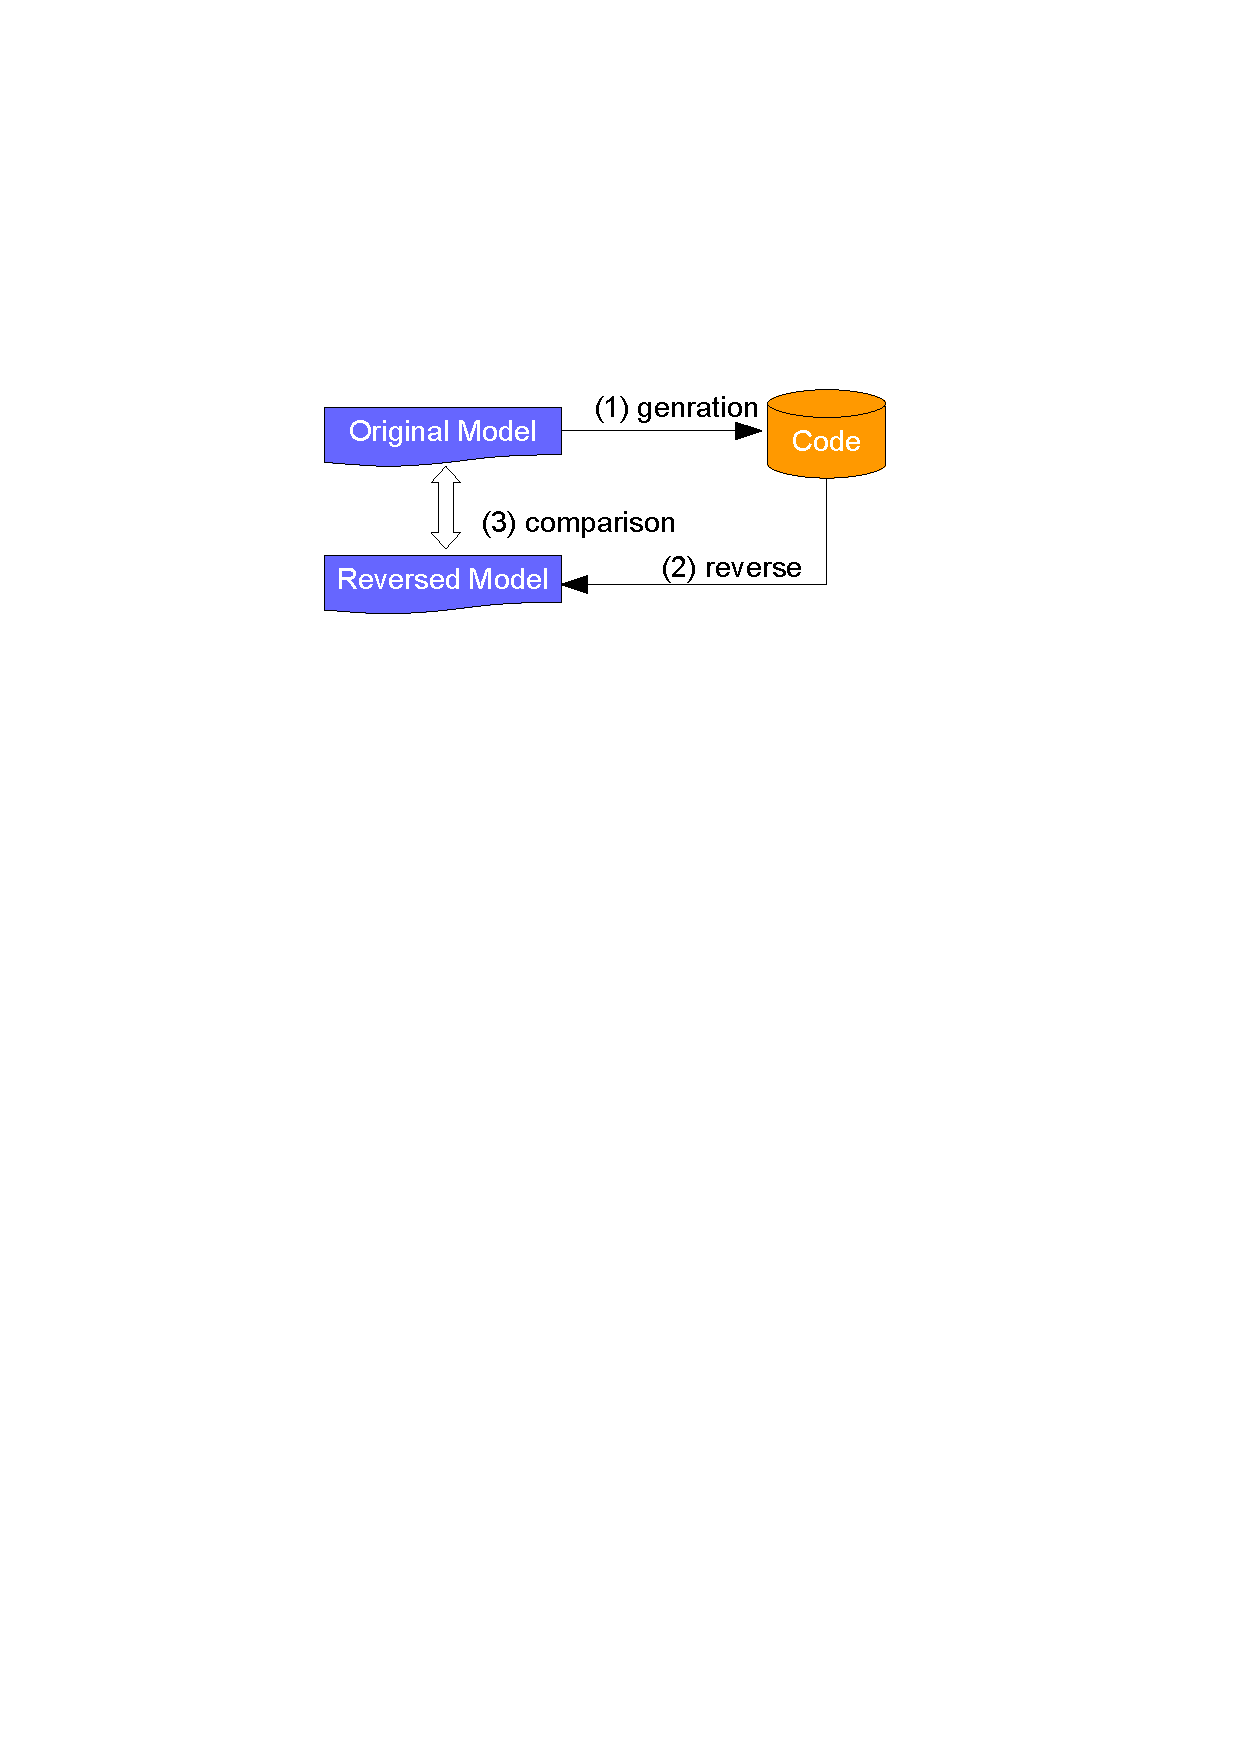
\includegraphics[clip, trim=5.5cm 19cm 5.5cm 6cm, width=0.3\textwidth]{figures/strategy1}
\caption{Evaluation methodology to answer RQ1} 
\label{fig:strategy1}
\end{figure}

\begin{figure}
\centering
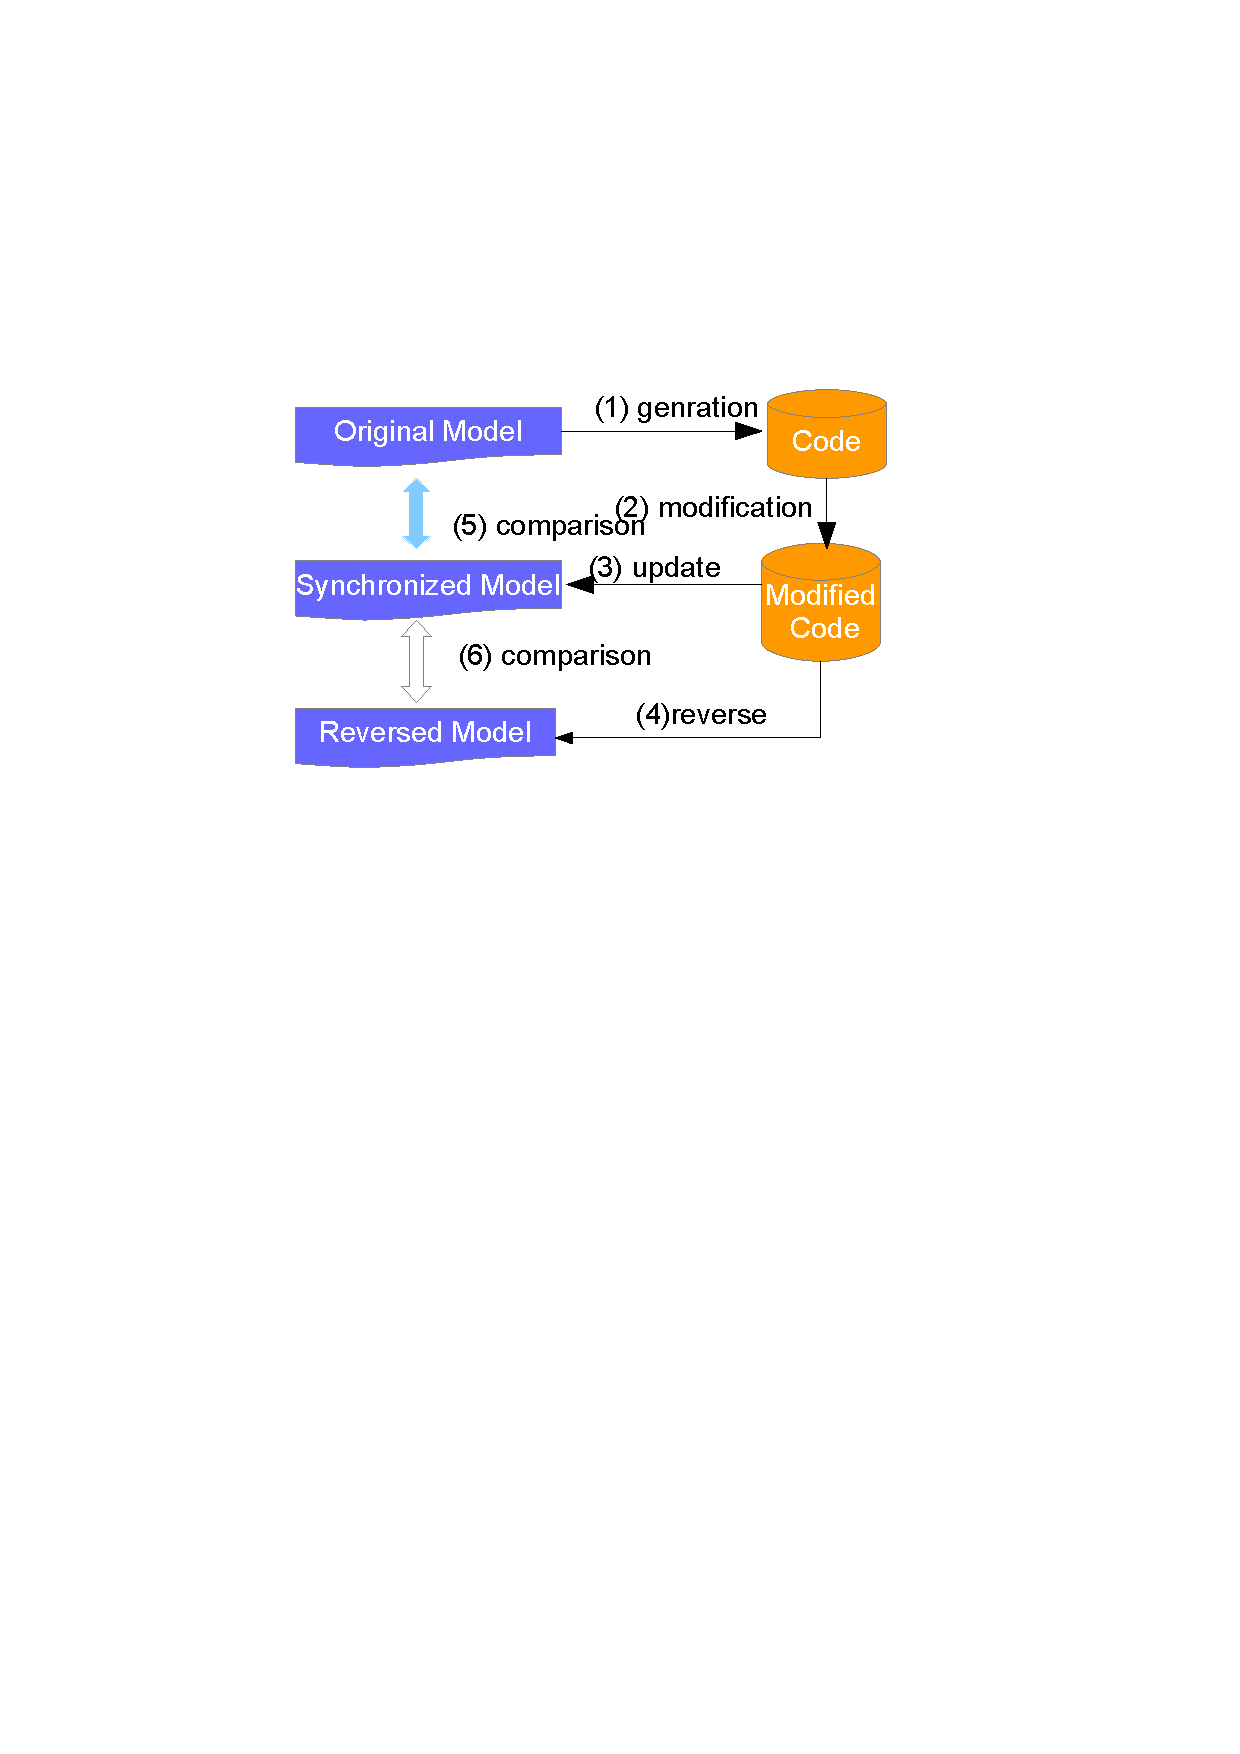
\includegraphics[clip, trim=4.5cm 16.5cm 5.5cm 6.5cm, width=0.3\textwidth]{figures/strategy2}
\caption{Evaluation methodology to answer RQ2} 
\label{fig:strategy2}
\end{figure}

Furthermore, in software development projects, some traditional programmers might want to practice with code in a traditional way and some MDE developers may prefer working with models. Therefore, it is necessary to compare the development/maintenance cost between the two practices by comparing the number of steps needed to do the same action. 


\subsection{Reversing generated code}
This experiment is targeting \tb{RQ1}. 300 hierarchical state machines are randomly automatically generated. Each of these has 80 states including atomic and composite states, and more than 234 transitions. The number of elements is unrealistically big but it is artificially used to show the scalability of the approach. The number of lines of generated code for each machine is around 13500. Names of the generated states are different. An initial pseudo state and a final state are generated for each composite state and containing state machine. Other elements such as call events, time events, transition/entry/exit actions and guards are associated with an appearance probability sensing that if a random number is less than the probability, the element associated with the probability is generated. For each generated call event, an operation is generated in the context class which is also generated. The duration is also generated for each time event. 


\begin{table}
\centering
\caption{Set-up information for model generation}
\label{table:setup}
\begin{tabular}{|l|l|}
\hline
Description                                     & Value            \\ \hline
Number of generated states                      & 80               \\ \hline
Number of generated transitions                 & \textgreater 234 \\ \hline
Probability of having an event for transition   & 0.8              \\ \hline
Probability of having CallEvent for transition  & 0.7              \\ \hline
Probability of having an entry/exit action for state & 0.7              \\ \hline
Probability of having a transition action and guard       & 0.7              \\ \hline
\end{tabular}
\end{table}

The set up information for the SM generation is shown in Table \ref{table:setup}. Code is generated from each state machine. The generated code is reversed to a state machine. The latter is then compared to the original one by using information of SM such as the number of states, transitions. 

\begin{table}
\centering
\caption{Model results of generation and reverse}
\label{table:law1-resultat}
\begin{tabular}{|l|l|l|l|l|}
\hline
Test ID & AS & CS & T & Is reverse correct? \\ \hline
1       & 47 & 33 & 234 & Yes                 \\ \hline
2       & 42 & 38 & 239 & Yes                 \\ \hline
3       & 43 & 37 & 238 & Yes                 \\ \hline
..      & .. & .. & .. & Yes                 \\ \hline
300       & 41 & 39 &240 & Yes                 \\ \hline
\end{tabular}
\end{table}
 
 
\begin{comment}
\begin{table*}[]
\centering
\caption{MODEL RESULTS OF GENERATION AND REVERSE}
\label{table:law1-resultat}
\begin{tabular}{|l|l|l|l|l|l|l|l|l|l|l|l|l|l|}
\hline
Test ID & AS & CS & D  & T   & EA & ExA & TA  & CE  & TE & G   & I  &    & Is reverse correct? \\ \hline
1       & 47 & 33 & 8  & 234 & 53 & 50  & 149 & 145 & 40 & 147 & 34 & 25 & Yes                 \\ \hline
2       & 42 & 38 & 8  & 239 & 52 & 59  & 165 & 145 & 36 & 133 & 39 & 31 & Yes                 \\ \hline
3       & 43 & 37 & 7  & 238 & 54 & 59  & 159 & 141 & 34 & 145 & 38 & 28 & Yes                 \\ \hline
..      & .. & .. & .. & ..  & .. & ..  & ..  & ..  & .. & ..  & .. & .. & Yes                 \\ \hline
300       & 41 & 39 & 10 & 240 & 56 & 55  & 165 & 142 & 37 & 151 & 40 & 33 & Yes                 \\ \hline
\end{tabular}
\end{table*}
\end{comment}

Table \ref{table:law1-resultat} shows some of the generated models which have the same information as the models created by doing the backward process of the generated codes. The number of atomic states (\tb{AS}), composite states (\tb{CS}), transitions (\tb{T}) are shown in Table \ref{table:law1-resultat}. The results of this experiment show that the proposed approach and the implementation can successfully do code generation from state machines and reverse. The answer to \tb{RQ1} is Yes. 

\subsection{Change propagation} 
A state machine (model level) describing Java Thread life-cycle \cite{_java_thread} and another one representing a telephone presented in \cite{Specification2007} are manually created. For each SM code is generated. Code is then manually modified by several actions described in Table \ref{table:cost}. The original SM is updated by doing a backward process from the modified generated code with the presence of the intermediate and original model. The updated SM is in turn compared with the SM created by the reverse engineering (see Fig. \ref{fig:strategy2}). 

\begin{table}
\centering
\caption{Change propagation experimental results}
\label{table:change-propa}
\begin{tabular}{|l|l|l|l|l|}
\hline
Test ID & Changes & Original & Updated & Reversed \\ \hline
1       &         &          &         &          \\ \hline
2       &         &          &         &          \\ \hline
3       &         &          &         &          \\ \hline
4       &         &          &         &          \\ \hline
\end{tabular}
\end{table}

\subsection{Time complexity and performance}
We are interested in knowing which element type among state, transition and event dominates the running time of the reverse engineering in case of creating new SM from code. To analyze the time complexity, we consider two tasks: semantic verification and SM construction from the verification output. Let us use the following parameters of the input SM used in code generation: $n_{s}$ = number of states, $n_{t}$ = number of transitions, $n_{ce}$ = number of call events, $n_{te}$ = number of time events, $n_{a}$ = number of actions and guards including entry/exit/transition actions and guards which are all implemented in the context class. 

For each state, the semantic verification consists of several phases as followings: (1) detecting composite/sub-state pattern, (2) loop over all methods of a state class, (3) detecting entry action pattern, (4) detecting exit action pattern, (5) detecting processing \ti{CallEvent}, (6) detecting processing \ti{TimeEvent}, and (7) detecting default state pattern. 
\begin{comment}
\begin{itemize}
  \item Detecting composite/sub-state pattern: $C_{childParentPattern} = ns^2 = O (ns^2)$.
  \item Loop over all methods of a state class: $CfindAllStateOperation = ns + nce + nt$. 
  \item Detecting entry action pattern: $Centry = na + CverifyTransition + CfindFunctionDefinition 
      = 6ns + 6nce + 5na + nt$
   \item Detecting exit action pattern: Cexit = 3nce + 3ns + 3na + nt
   \item Detecting processing CallEvent: CprocessEvent = 7nce + 6ns + 2nt + 2na 
   \item Detecting processing TimeEvent: CprocessTimeEvent = 6nce + 6ns + 2nt + 2na
   \item Detecting default state pattern: CsetInitDefaultState = 3nce + 3ns + nt + na
\end{itemize}

\begin{itemize}
  \item Detecting composite/sub-state pattern
  \item Loop over all methods of a state class
  \item Detecting entry action pattern
   \item Detecting exit action pattern
   \item Detecting processing \ti{CallEvent}
   \item Detecting processing \ti{TimeEvent}
   \item Detecting default state pattern
\end{itemize}
\end{comment}
Since the space is limited, we cannot present the detail of the complexity of each phase. To sum up, the semantic verification has a worst-case complexity $C_{1} = n_{s}(n_{s^2} + 9n_{t^2} + 6n_{t}n_{s} + 2n_{a}n_{ce}) = O (n_{s^3}) + O (n_{t}n_{s^2}) + O (n_{s}n_{t^2}) = O (n^3)$ with $n = max (n_{t}, n_{s})$. The worst-case occurs if a state can accept all incoming events and all transitions have the same source state. This is indeed unrealistic.

The SM construction from the verification output has a worst-case time complexity $C_{2} = O (n_{s^2}) + O (n_{s} n_{t}) = O (n_{^2})$. Therefore, the reverse engineering has a worst-case complexity of $O (n^3)$ with $n = max (n_{s}, n_{t})$.

To analyze the performance of reverse engineering, we randomly generate 5 models with base set up information in which the numbers of states and transitions are 20 and 50, respectively. We use a Dell Latitude E554 laptop with a 2.1GHz Intel Core i7 with 16 Gb of RAM. The running time of the reverse for the generated code associated with these models is measured. To analyze the impact of state and transition to the reverse performance, we change the set up information by increasing either the number of states or transitions, and keep intact the other. The increase is of 5, 10, 15, and so on. The models resulting from the modifications are used for generating code. The running time of reverse engineering the new generated code is measured. For each measurement, three times are computed, the median of these measured values are retained. 

\begin{table}
\centering
\caption{Time measurements}
\label{table:time-measurment}
\begin{tabular}{|l|l|l|l|}
\hline
Increase & Original & State  & Transition \\ \hline
5        & 64557    & 78021  & 62271      \\ \hline
10       & 64557    & 83025  & 68374      \\ \hline
15       & 64557    & 96761  & 64176      \\ \hline
20       & 64557    & 118879 & 71728      \\ \hline
25       & 64557    & 132763 & 73445      \\ \hline
30       & 64557    & 153120 & 75314      \\ \hline
35       & 64557    & 163538 & 78647      \\ \hline
40       & 64557    & 185361 & 81547      \\ \hline
\end{tabular}
\end{table}

Table \ref{table:time-measurment} shows the increase of the number of instances for states and transitions and the execution time of the original and modified models. The results show that when the number of states has more impact to the performance overall than the number of transitions. Figure \ref{fig:graph} also shows clearer the comparison of performance between the original model, the models modified by adding states and transitions. When the number of added states grows, the running time for reverse also grows quickly. Whereas, in case of transitions, the difference is small and not clear as we analyze that the worst-case complexity never occurs.

\begin{figure}
\centering
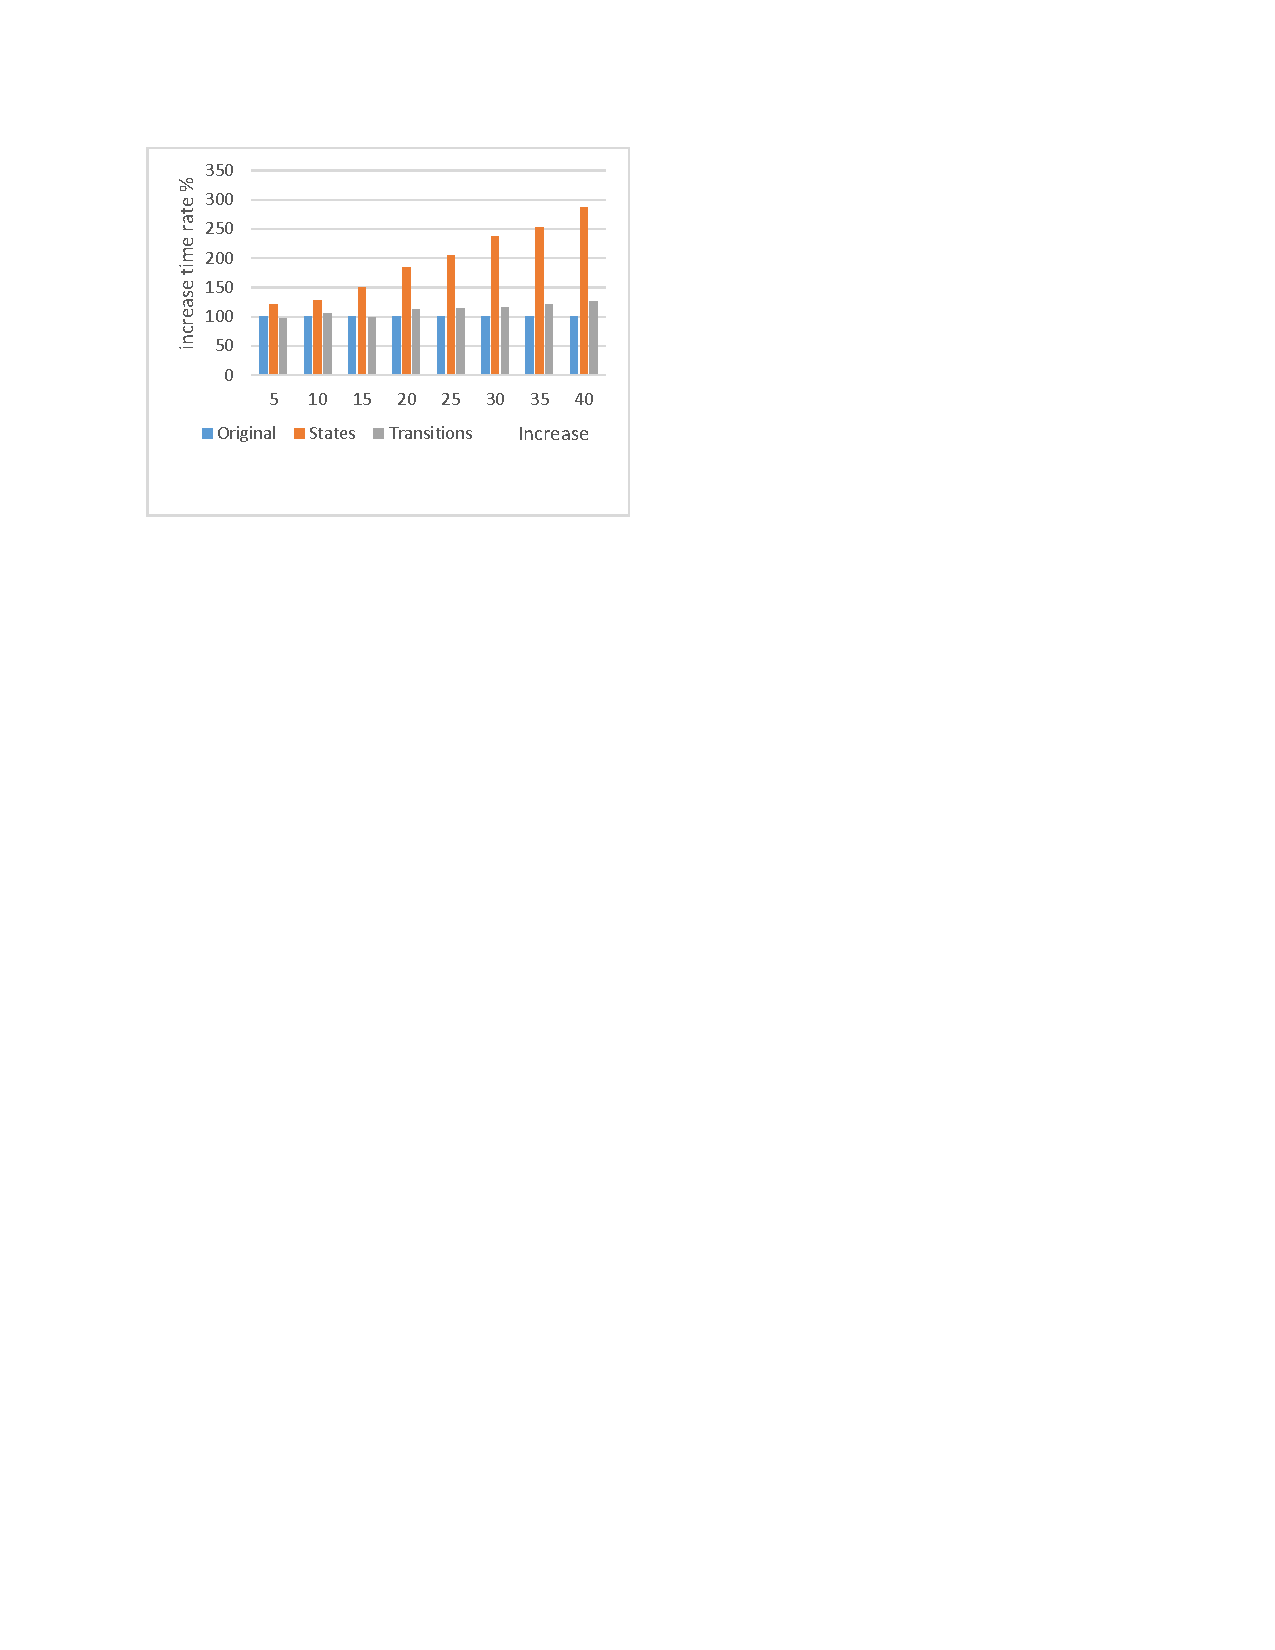
\includegraphics[clip, trim=3cm 20.5cm 11cm 2.6cm, width=0.5\textwidth]{figures/graph}
\caption{Impact comparison between states and transitions} 
\label{fig:graph}
\end{figure}

\subsection{Semantic conformance of runtime execution}
To evaluate the semantic conformance of runtime execution of generated code, we use a set of examples provided by Moka [XXX] which is a model execution engine offering Precise Semantics of UML Composite Structures \cite{OMG2015}. We compare the entered-ordered state list, which is obtained by simulating a state machine with the engine, with the state list obtained by the runtime execution of the generated code of the same state machine. The generated code is semantic-conformant if both of the lists are the same. [To be continued]

\subsection{Development/maintenance cost}
\label{subsec:cost}
To compare the development/maintenance cost, we investigate steps needed in generated code and models having the equivalent semantics. For example, to add a state, on one hand, two steps are needed in diagrams including (1) specifying the parent state and (2) dragging \& dropping the state notation to that parent. On the other hand, three code modifications are (1) create a state class inheriting from the base state and its constructors, (2) add to the parent state class an attribute, and (3) add a line of code to initialize the state attribute in the parent state constructor. Table \ref{table:cost} shows the number of steps needed for each operation. In this table, model manipulations are the winner in most of cases because of graphical representation advantages but code manipulations are still useful and comparable.

\begin{table}
\centering
\caption{Cost comparison}
\label{table:cost}
\begin{tabular}{|l|l|l|}
\hline
Description                                     & Model & Code \\ \hline
Add a state                                     & 2     & 3    \\ \hline
Add a transition                                & 3     & 3    \\ \hline
Add entry/exit action                           & 2     & 2    \\ \hline
Add transition action                           & 2     & 2    \\ \hline
Update action                                   & 1     & 1    \\ \hline
Redirect target state of a transition           & 1     & 1    \\ \hline
Create a call event to a transition & 3     & 6    \\ \hline
Create a time event to a transition & 3     & 5    \\ \hline
Delete a state                                  & 2     & 2    \\ \hline
Delete a transition                             & 1     & 3    \\ \hline
Delete entry/exit action                        & 1     & 2    \\ \hline
Delete transition action                        & 1     & 2    \\ \hline
Delete a call event                             & 2     & many \\ \hline
Delete a time event                             & 2     & many \\ \hline
\end{tabular}
\end{table}

In software development, programmers might modify the generated code, the modifications might violate structures of code or SM semantics. To resolve this issue, as previously described, we provide a semantic verification that partly and loosely inspects the AST of generated code. This inspection approach always reverses the code to the SM as well as the code is state machine-compliant even though the code is not compiled. This approach is very useful in practice in which programmers might partly modify code, automatically update the original SM by our RTRIP, and automatically re-generate state machine-compliant code into the remaining application code. This re-generation does no more than completing missing elements in code meaning that all previous changes are preserved. This practice is also limitedly supported by Fujaba \cite{KNNZ99_2_ag} in which activity and collaboration diagrams are partly synchronized with JAVA.



